\section{Computer Vision}
\label{sec:vision}
Various vision algorithms are needed for more careful perception and analysis of Pepper's environment on object and huamn level. 
To start interaction, our Pepper can detect and recognize different people, remember their names and some other features, and track them using its camera data. 
Then, more interested skills will be shown to carry more complex tasks. For example, some tasks require human posture recognition so an algorithm based on OpenPose \cite{Cao_2017_CVPR} is developed. 
It can recognize human skeleton so that we can judge whether a person is standing, sitting or pointing somewhere. For object-level environment reasoning, we build a detection and recognition framework based on YOLO \cite{Redmon2018YOLOv3AI}, an interesting real-time algorithm. 
According to the competition environment of RobCup@Home, our framework can detect 50 classes of indoor objects in real time and print its name in the figure.
To train our object detection network, we made a dataset containing 50 classes indoor objects from OpenImages.We also matched adjacent input frames to make the detection more robust.
In some detection tasks we need a large field of view, but the top 2D camera makes us disappointed. So we need to take some measures to expand Pepper's limited original "eyes".
The method we choose is to stitch images from fifferent perspectives, and a fusion algorithm follows to reduce the influence of illumination and geometric change.
Now more visual candidates are included for further processing.
\begin{figure}[h!]
\centering
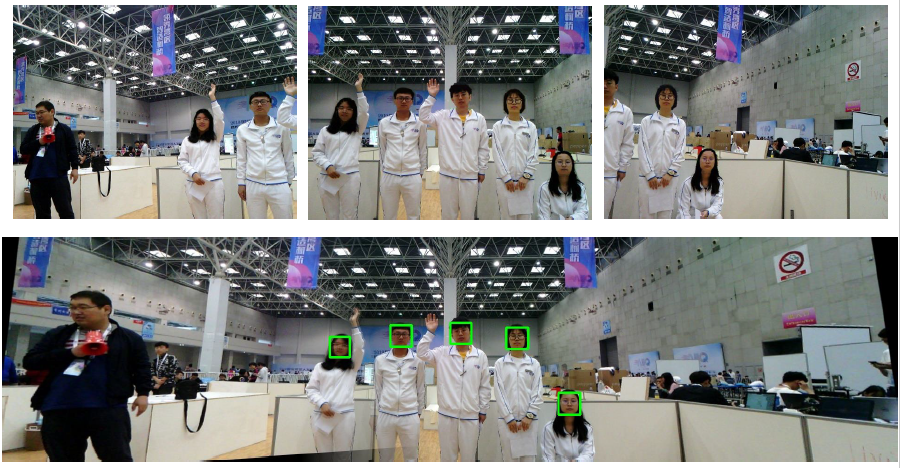
\includegraphics[width=1.\textwidth]{figs/vision1.png}
\caption{Image Stitch and Fusion to Detect in a Lager Field of View}
\label{fig:vision1}
\end{figure}
Now we are trying to expand the visual functions like person's pose estimation. 
For person's pose estimation,we use OpenPose model to perform multi-person pose estimation. 
The main steps of this method are input image stream, predict confidence map for body part detection and vector fields of part affinities, then clustering the key points to matching associate body parts, and finally assemble them into full body pose in image. 
\begin{figure}[h!]
    \centering
    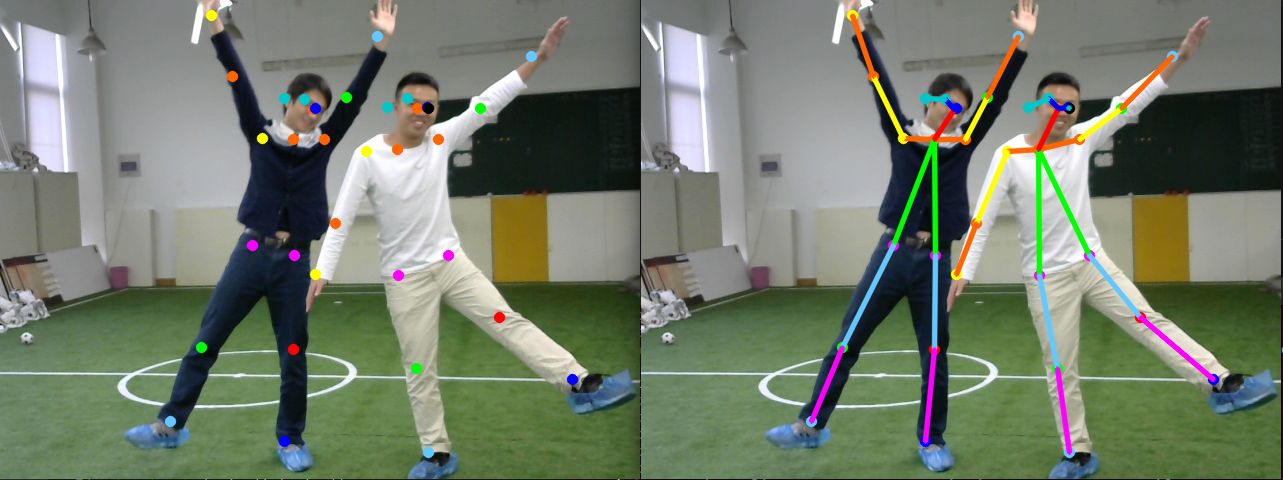
\includegraphics[width=1.\textwidth]{figs/vision2.png}
    \caption{Using OpenPose model to estimate body pose}
    \label{fig:vision2}
    \end{figure}

The Naoqi framework contains many useful APIs,so we take advantages of them. 
For vision part,we can use API to judge person whether standing or sitting, whether close or far away from robot. 
They can also analyze person's expression and clothes color. These functions are integrated to human-robot interaction module.